%%%%%%%%%%%%%%%%%%%%%%%%%%%%%%%%%%%%%%%%%%%%%%%%%%%%%%%
%                   File: OSAmeetings.tex             %
%                  Date: 29 Novemver 2018              %
%                                                     %
%     For preparing LaTeX manuscripts for submission  %
%       submission to OSA meetings and conferences    %
%                                                     %
%       (c) 2018 Optical Society of America           %
%%%%%%%%%%%%%%%%%%%%%%%%%%%%%%%%%%%%%%%%%%%%%%%%%%%%%%%

\documentclass[letterpaper,10pt]{article}
%% if A4 paper needed, change letterpaper to A4

\usepackage{osameet3} %% use version 3 for proper copyright statement

%% standard packages and arguments should be modified as needed
\usepackage{amsmath,amssymb}
\usepackage[colorlinks=true,bookmarks=false,citecolor=blue,urlcolor=blue]{hyperref} %pdflatex
%\usepackage[breaklinks,colorlinks=true,bookmarks=false,citecolor=blue,urlcolor=blue]{hyperref} %latex w/dvipdf
\usepackage{subfigure}

\begin{document}

\title{Phase shift extraction algorithm based on PCA method in Digital Holographic Microscopy under Structured Illumination}

\author{Da Yin$^1$,Caojin Yuan$^{1,*}$}
\address{$^1$Key Laboratory for Opto-Electronic Technology of Jiangsu Province, Nanjing Normal University, Nanjing, 210023, China}
\email{$^*$yuancj@njnu.edu.cn}

%% Uncomment the following line to override copyright year from the default current year.
\copyrightyear{2019}


\begin{abstract}
%In this paper,We present a phase shift extraction algorithm to improve the resolution of digital holographic microscopy (DHM) under the structured illumination (SI) based on principal component analysis(PCA) method.
%Meanwhile,The modulated frequency of SI and the quadratic phase can be easily removed from the recorded infornmation by the PCA algorithm.
%Both the simulation calculation and experiment show that the phase shifts with high precision can be determined with the proposed PCA algorithm easily.
We present a phase shift extraction algorithm in digital holographic microscopy under structured illumination based on principal component analysis(PCA) method.
The experinments is obtained satisfactory results by this method and shows $78\%$ resolution improvement.
\end{abstract}

\ocis {(090.1995) Digital holography; (100.6640) Superresolution}

\section{Introduction}
In recent years,digital holographic microscopy (DHM) as a powerful tool for amplitude-contrast and phase-contrast imaging has been used in biomedical imaging.
The structured illumination (SI) is one of methods to overpass the diffraction limit in DHM\cite{Mico2006}.
%When SI is used in DHM, each direction of the illumination fringe is required to be shifted at least three times with known phase shift to perform the phase-shifting reconstruction.
%Other phase-shifting algorithms without any prior knowledge about the phase steps are iterative and require considerable computeraion\cite{Zheng2014}.
By using SI, three images with known phase-shifting amount are required to separate low and high frequency information in each direction.
Although iteration algorithm helps to retrieve the unknown phase-shifting amount, it is time-consuming and requires considerable computeraion\cite{Zheng2014}.

In this paper, we propose a phase-shifting extraction algorithm based on PCA method with unknown phase-shifting which is very fast and easy to implement.
We carry out the experiments to testify this method and obtain satisfactory results.

\section{Principle and Experimental results}
\begin{figure}[h]
    \centering
    \subfigure[]{
        \begin{minipage}[t]{0.5\linewidth}
        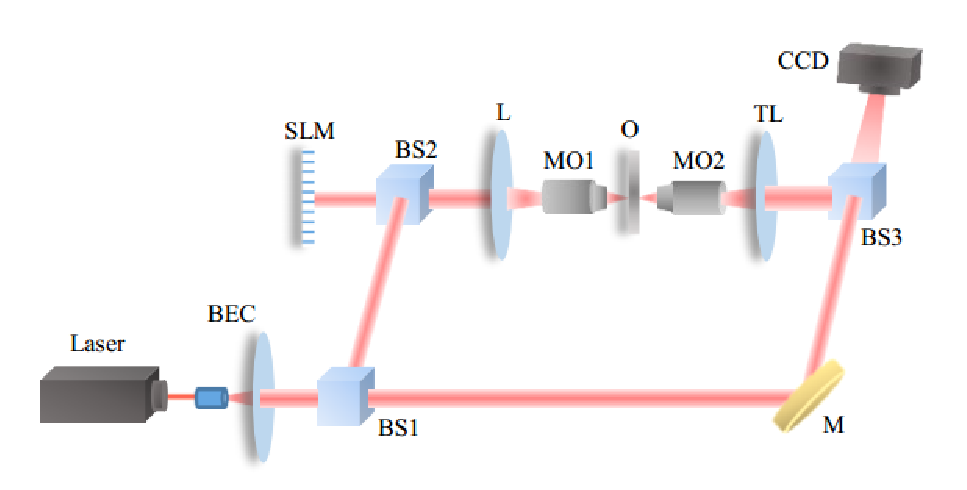
\includegraphics[height=1.5in]{path.eps}
        \label{fig:SystemPath}
        \end{minipage}
    }
    \subfigure[]{
        \begin{minipage}[t]{0.35\linewidth}
        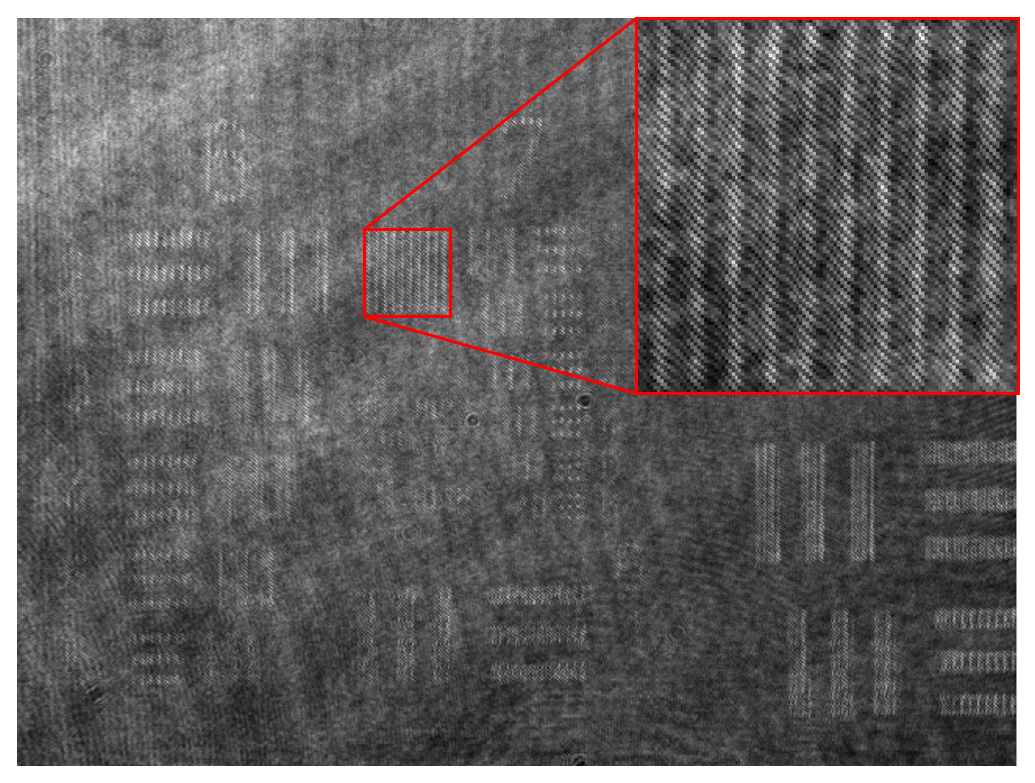
\includegraphics[height=1.5in]{hologram.eps}
        \label{fig:hologram}%
        \end{minipage}
    }  
    \centering
    \caption{The experiment steup of the SI-DHM system (a), First hologram $I_1$ of the SI-DHM (b)}
\end{figure}
The light from He-Ne laser with $\lambda=632nm$ is employed to illuminate the system of Fig. \ref{fig:SystemPath}.
The light is divided into two beams by a beam splitter(BS1).
One beam is used as the reference beam.
The other beam served as the object beam is reflected by BS2 and modulated by the spatial light modulator (SLM).
For each orientation the phase gratings loaded on SLM are shifted at least three times.
After extracting the $+1$st order from the hologram, the intensity of the projection as shown in Fig. \ref{fig:hologram}, which can be written as
\begin{eqnarray}
 I_{n}(x,y) = a(x,y) + b(x,y)cos[ \Phi(x,y) + \delta_n ] \label{Eq:intensity}
\end{eqnarray}
where $a(x,y)$ is the background illumination, $b(x,y)$ and $\Phi(x,y)$ are the modulation and the phase maps, respectively.
$\delta_n$ are the unknown phase steps, where $n$ denotes the phase-shifting index.
The red square in Fig. \ref{fig:hologram} is zoomed to show two interference patterns.

The PCA is a technique from statistics for reducing the dimensionality of an image or date set\cite{Vargas2011}.
According to the analysis in Eq (\ref{Eq:intensity}), suppose that we have constructed N images for each direction.
Each image set can be expressed in a matrix form as $X = [I_1,I_2,\cdots,I_N]^{T}$, where $[\cdot]^T$ denotes the transposing operation.
%\begin{eqnarray}
%X = [I_1,I_2,\cdots,I_N]^{T} \label{imageSets}
%\end{eqnarray}
%In the Eq (\ref{imageSets}), $[\cdot]^T$ denotes the transposing operation.

Taking into account the background is a smooth signal, we can estimate $X_m = \frac{1}{N}\sum_{n=1}^{n=N}I_n$, where $X_m$ is the mean value of N images.
%\begin{eqnarray}
%X_m = \frac{1}{N}\sum_{n=1}^{n=N}I_n \label{Eq:MeanValue}
%\end{eqnarray}
%In probability theory and statistics, covariance matrix is a measure of the degree of linear correlation between two variables.
The covariance matrix C from X for PCA algorithm can be written as $C = [X - X_m][X-X_m]^T$.
%\begin{eqnarray}
%C = [X - X_m][X-X_m]^T \label{Eq:covariance}
%\end{eqnarray}
%The covariance matrix C can represent the data in a compact way.
In practically, $X-X_m$ represent a background suppression operation.
Covariance matrix C is decomposed into eigenvalues $V$ and eigenvectors $Q$.
From matrix theory, we can express it as $CQ = VQ$.
%\begin{eqnarray}
%CQ = VQ \label{Eq:eig}
%\end{eqnarray}
As an orthogonal matrix, Q can be constructed by $Q=[Q_1,Q_2,\cdots,Q_N]^T$.
The covariance matrix C Can be diagonalized as $D = Q^TCQ$.
%\begin{eqnarray}
%D = Q^TCQ \label{Eq:SVD}
%\end{eqnarray}
D is a diagonal matrix comprised by the eigenvalues V.
%This diagonalization process is achieved by the singular value decomposition (SVD) algorithm in PCA method.
Through the covariance matrix C and the orthogonal matrix Q, we can extract the principal components as
\begin{eqnarray}
\Psi = Q(X-X_m) = [Q_1,Q_2,\cdots,Q_N]^T(X-X_m) \label{Eq:Hotelling}
\end{eqnarray}
where $\Psi=[\Psi_1,\Psi_2,\cdots,\Psi_N]$ are the principle components of the $X-X_m$.
We can extract two uncorrelated quadrature signal $I_c(x,y) = b(x,y)cos[\Phi(x,y)]$ and $I_s = b(x,y)sin[\Phi(x,y)]$ from $\Psi$ corresponded to the biggest eigenvalues ($\Psi_1$ and $\Psi_2$).
Thus the $-1$st diffraction order $I_L$ and $+1$st diffraction order $I_R$ can be extracted from the image set in each direction.
The two orders can be estimated as $FT(I_L) = FT(I_s) - iFT(I_c) \quad and \quad FT(I_R) = FT(I_s) + iFT(I_c)$.
%\begin{eqnarray}
%FT(I_L) = FT(I_s) - iFT(I_c) \quad and \quad FT(I_R) = FT(I_s) + iFT(I_c) \label{Eq:Hilbert}
%\end{eqnarray}
where $FT$ denotes the Fourier transform and $i = \sqrt{-1}$.

The next step is to assemble the $-1$st and $+1$st diffraction order in frequency domain in each direction.
%Thus the synthesized image can contain sub-resolution information.
In this experiment, we only use three images in horizontal direction and three images in vertical direction.
The information of Frequency domain in Fig.\ref{fig:structure} is consist of four diffraction order.
The normal microscopy image is shown in Fig.\ref{fig:raw} for the contrast, where the Group 8, Element 3 (323Lp/mm) in the USAF test target can be resolved.
The intensity distributions along the blue lines in the Group 9, Element 2 in Fig.\ref{fig:raw} and Fig.\ref{fig:structure} are plotted in Fig. \ref{fig:plot}.
It's clear that the resolution reaches 575Lp/mm with PCA method and it shows $78\%$ resolution improvement in experiment.

\begin{figure}[h]
    \centering
    \subfigure[]{
        \begin{minipage}[t]{0.31\textwidth}
            \centering
            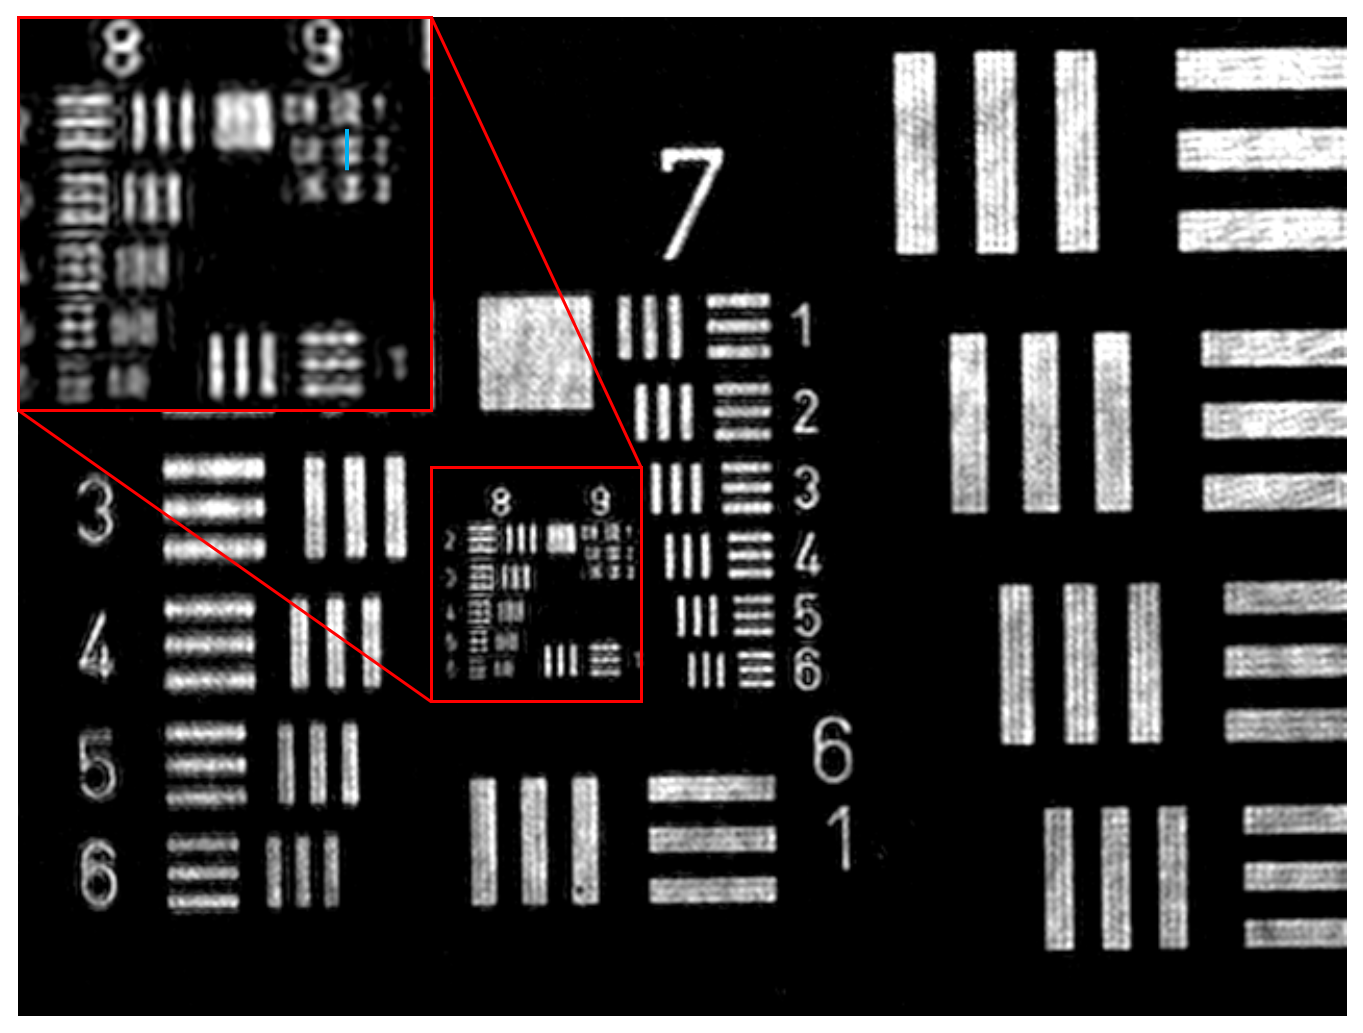
\includegraphics[width=2in]{raw.eps} \label{fig:raw}
        \end{minipage}
    }
    \subfigure[]{
        \begin{minipage}[t]{0.31\textwidth}
            \centering
            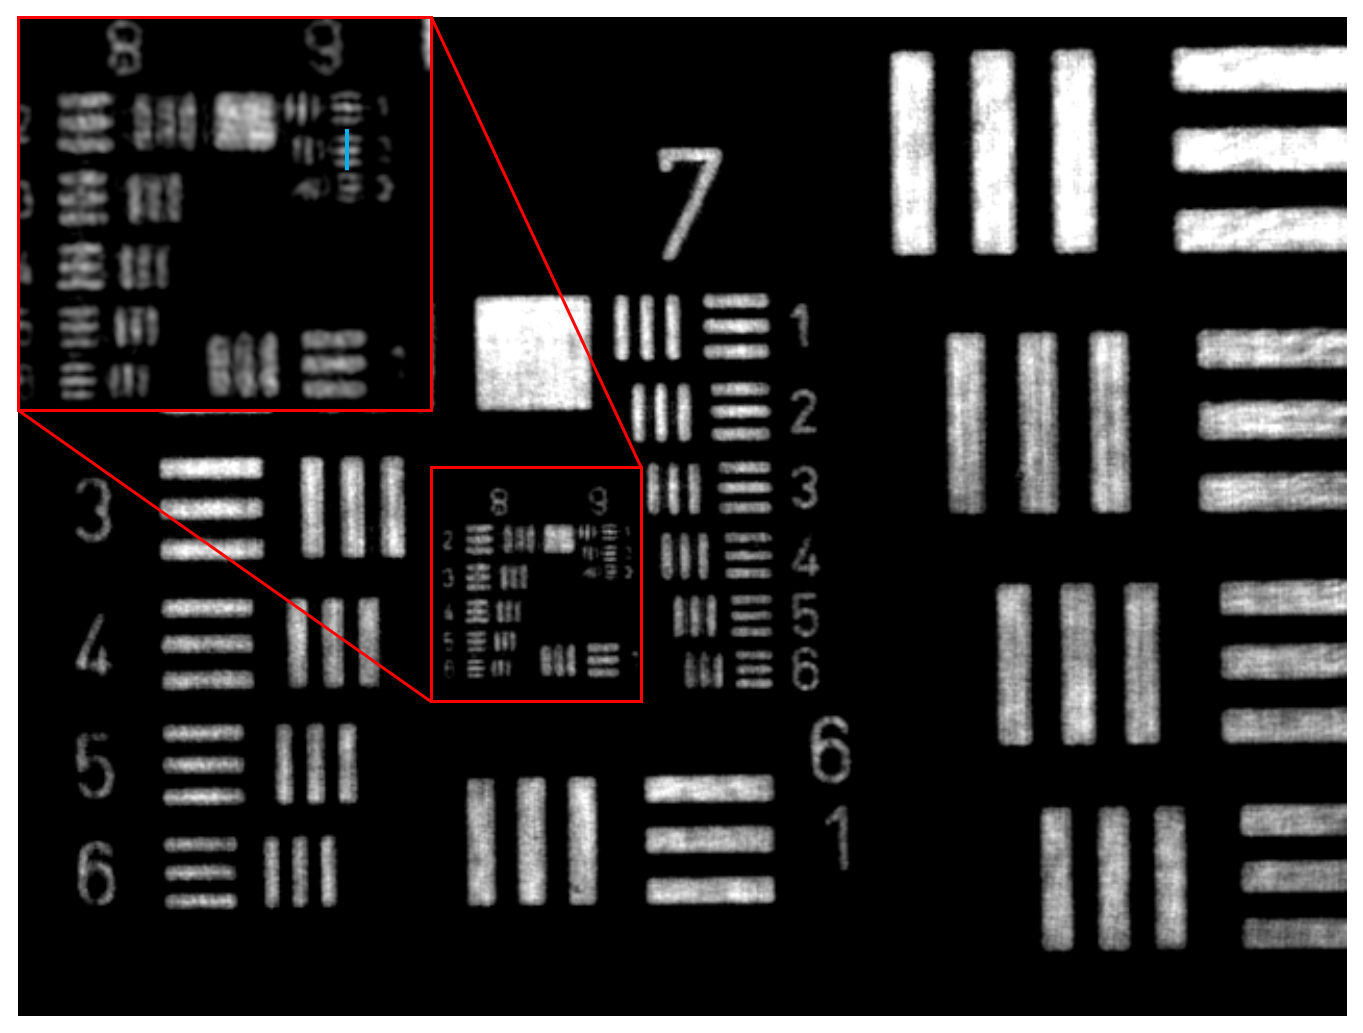
\includegraphics[width=2in]{structure.eps} \label{fig:structure}
        \end{minipage}
    }
    \subfigure[]{
        \begin{minipage}[t]{0.31\textwidth}
            \centering
            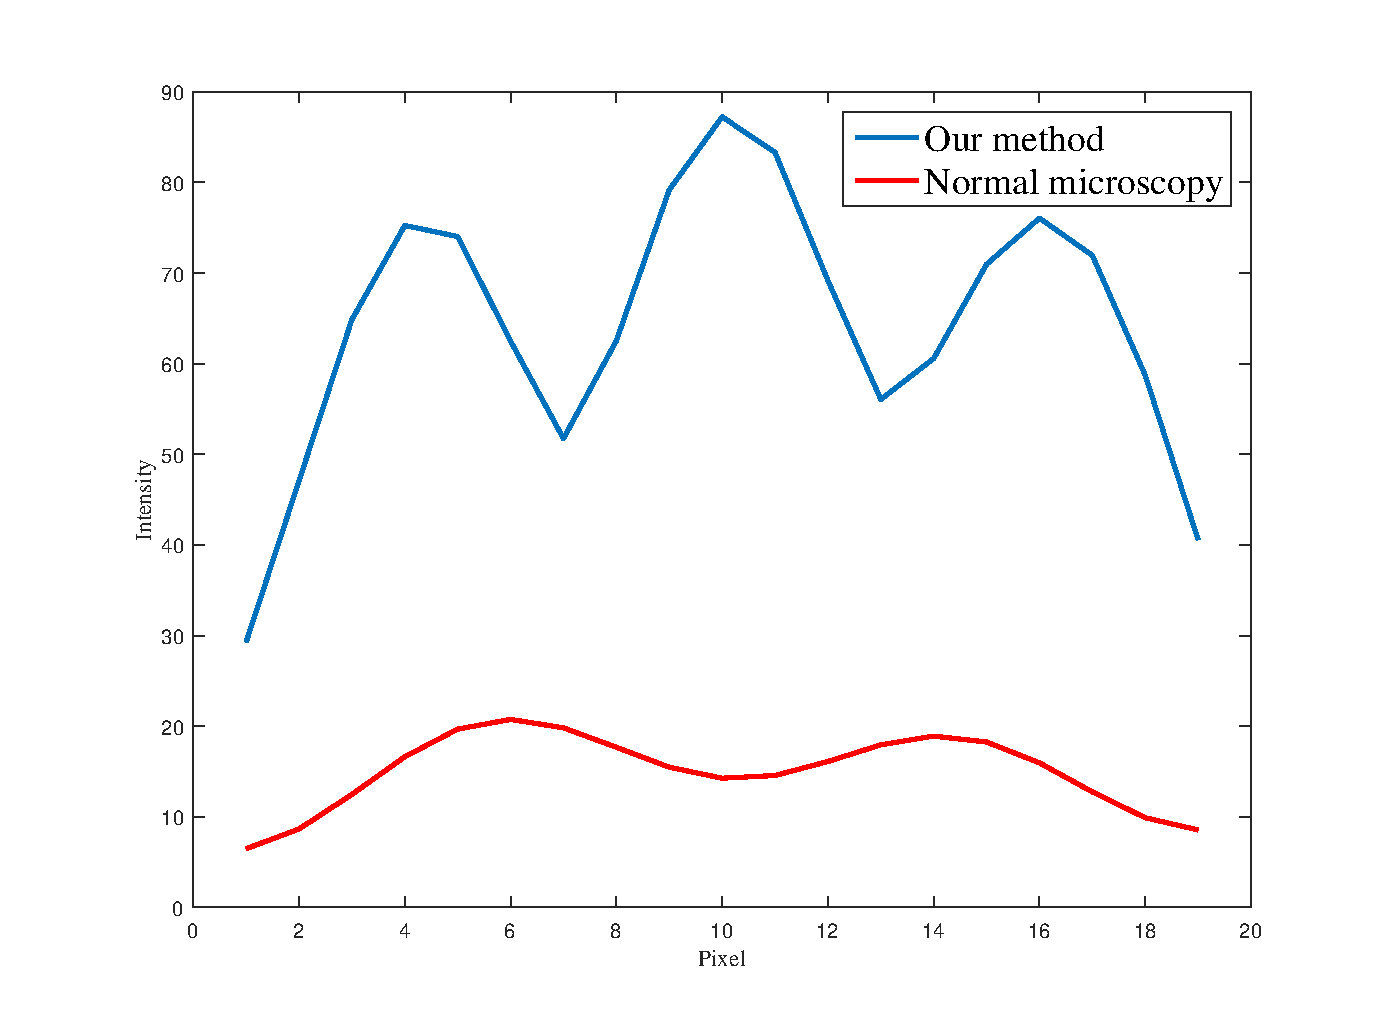
\includegraphics[width=2in]{plotLine.eps} \label{fig:plot}
        \end{minipage}
    }
    \centering
    \caption{Normal microscopy image (a), synthesized image (b), plots along the blue line of (a) and (b)}
\end{figure}

\section{Conclusion}
A new phase shift extraction algorithm in DHM under SI based on PCA method has been presented.
This method does not need any prior knowledge and the proposed method is fast and effectively.

\section{Acknowledgment}
This work is supported by the National Natural Science Foundation of China (NSFC) (61775097, 61605080).

\begin{thebibliography}{99} %% use BibTeX or add references manually

\bibitem{Mico2006} V. Mico, Z. Zalevsky, ``Synthetic aperture superresolution with multiple off-axis holograms,''
J. Opt. Soc. Am. A. \textbf{23}(12), 3162--3170 (2006).

\bibitem{Zheng2014} J. Zheng, P. Gao, B. Yao, T. Ye, J. Min, D. Dan, Y. Yang, S.Yan, ``Digital holographic microscopy with phase-shift-free structured illumination,''
Photonics Res. \textbf{2}(87), 1328--1330 (2013).

\bibitem{Vargas2011} J. Vargas, J. Antonio Quiroga, T. Belenguer, ``Phase-shifting interferometry based on principal component analysis,''
Opt. Lett. \textbf{36}(8), 1326--1328 (2011).

\end{thebibliography}


\end{document}
